\section{Results}

\subsection{Baseline Model}
\begin{scriptsize}
	\vspace{-\parskip}
	\url{https://wandb.ai/mfixman-convolutional-team/work/runs/j6iippi9}
	\hfill{} Wandb tag: `\texttt{baseline}'
\end{scriptsize}

The baseline model, being extremely simple, does nearly not overfit its data.
Instead, it badly underfits the data and doesn't give the best result.

\begin{figure}[h]
	\centering
	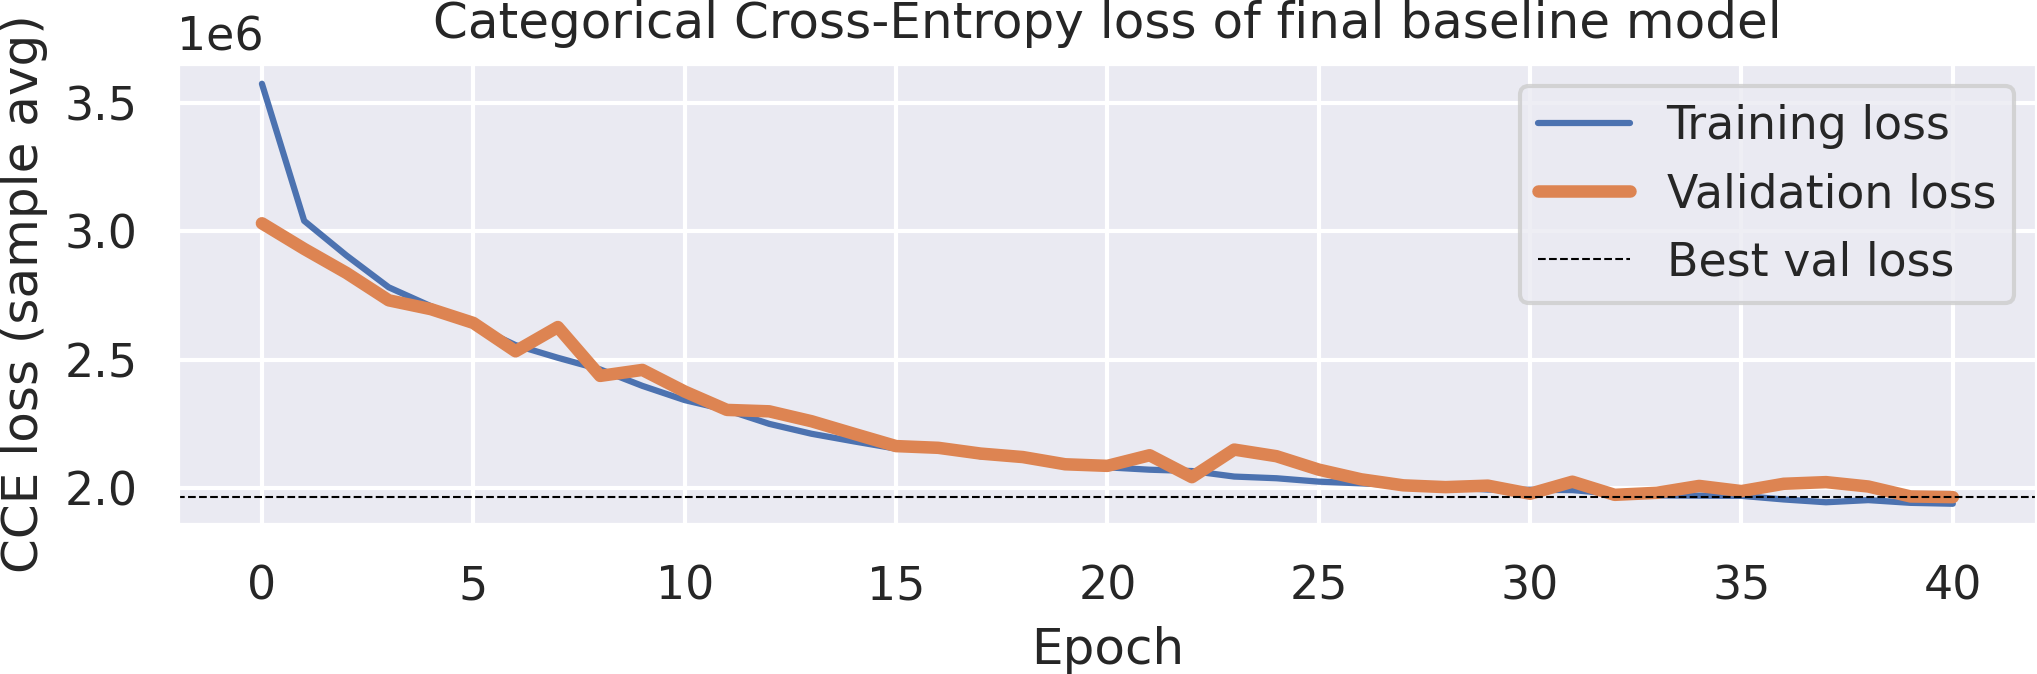
\includegraphics[width=.9\textwidth]{baseline_loss.png}
	\caption{Baseline loss by epoch}
\end{figure}

The results of this model are notoriously ``blocky'': while there are clusters of correct pixels where they should go, it seems the model has problems filling those clusters.
This is likely due to the small ratio between kernel size and minimum image, and the lack of skip connections which prevent it from nicely detecting the edges between different classes.

\begin{figure}[h]
	\begin{subfigure}{.5\textwidth}
		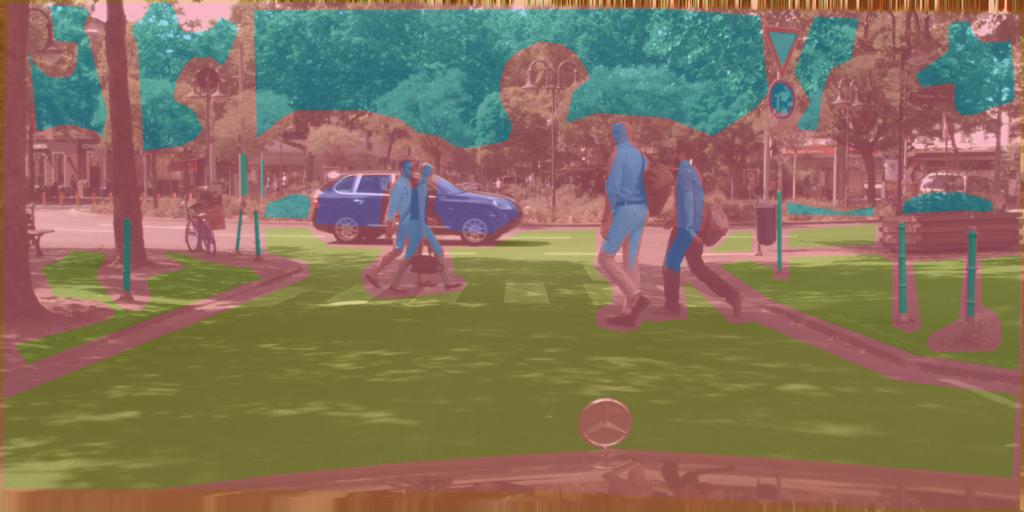
\includegraphics[width=\textwidth]{city_images/baseline_gt_pic.png}
		\caption{Ground truth}
	\end{subfigure}
	\begin{subfigure}{.5\textwidth}
		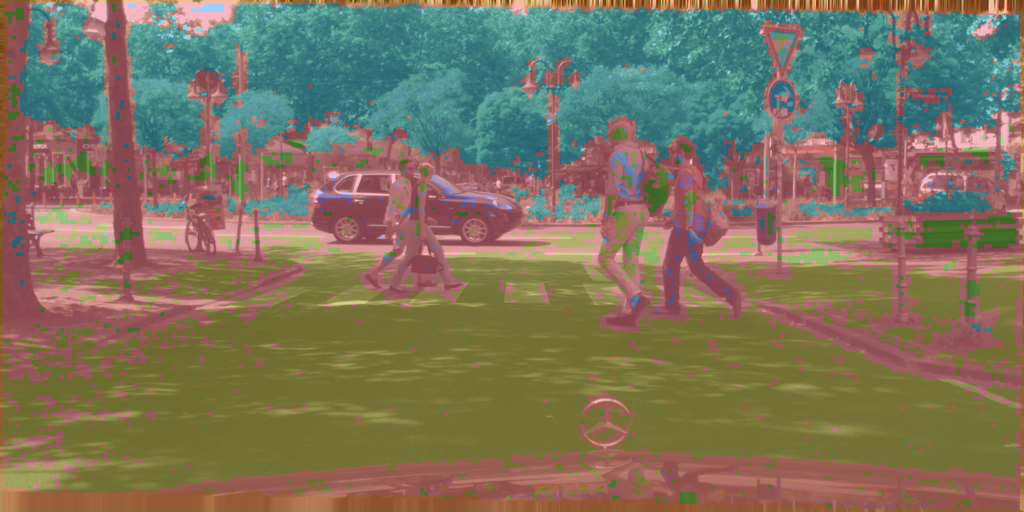
\includegraphics[width=\textwidth]{city_images/baseline_pic.png}
		\caption{Result of the baseline model.}
	\end{subfigure}
	\caption{Example result with a picture in the city of Frankfurt.}
\end{figure}

While the results are far from convincing, this works very well as a simple and light model: in this example and many others all objects (cars, people, trees, and others) are identified, regardless of how small.

It's also a fantastic starting point for a comparison.

\newpage{}

\subsection{Enhanced Model 1: UNet}
\begin{scriptsize}
	\vspace{-\parskip}
	\url{https://wandb.ai/mfixman-convolutional-team/work/runs/5ytrv216}
	\hfill{} Wandb tag: `\texttt{enhanced\_unet}' \\[-4pt]
	\url{https://wandb.ai/mfixman-convolutional-team/work/runs/qbi7duzd}\footnotemark{}
	\footnotetext{The original run got preempted and was later continued; the section shows both runs together.}
\end{scriptsize}

While the UNet model has considerably better loss than the baseline model, it overfits badly after only 15 epochs and doesn't learn much useful information afterwards.

\begin{figure}[h]
	\centering
	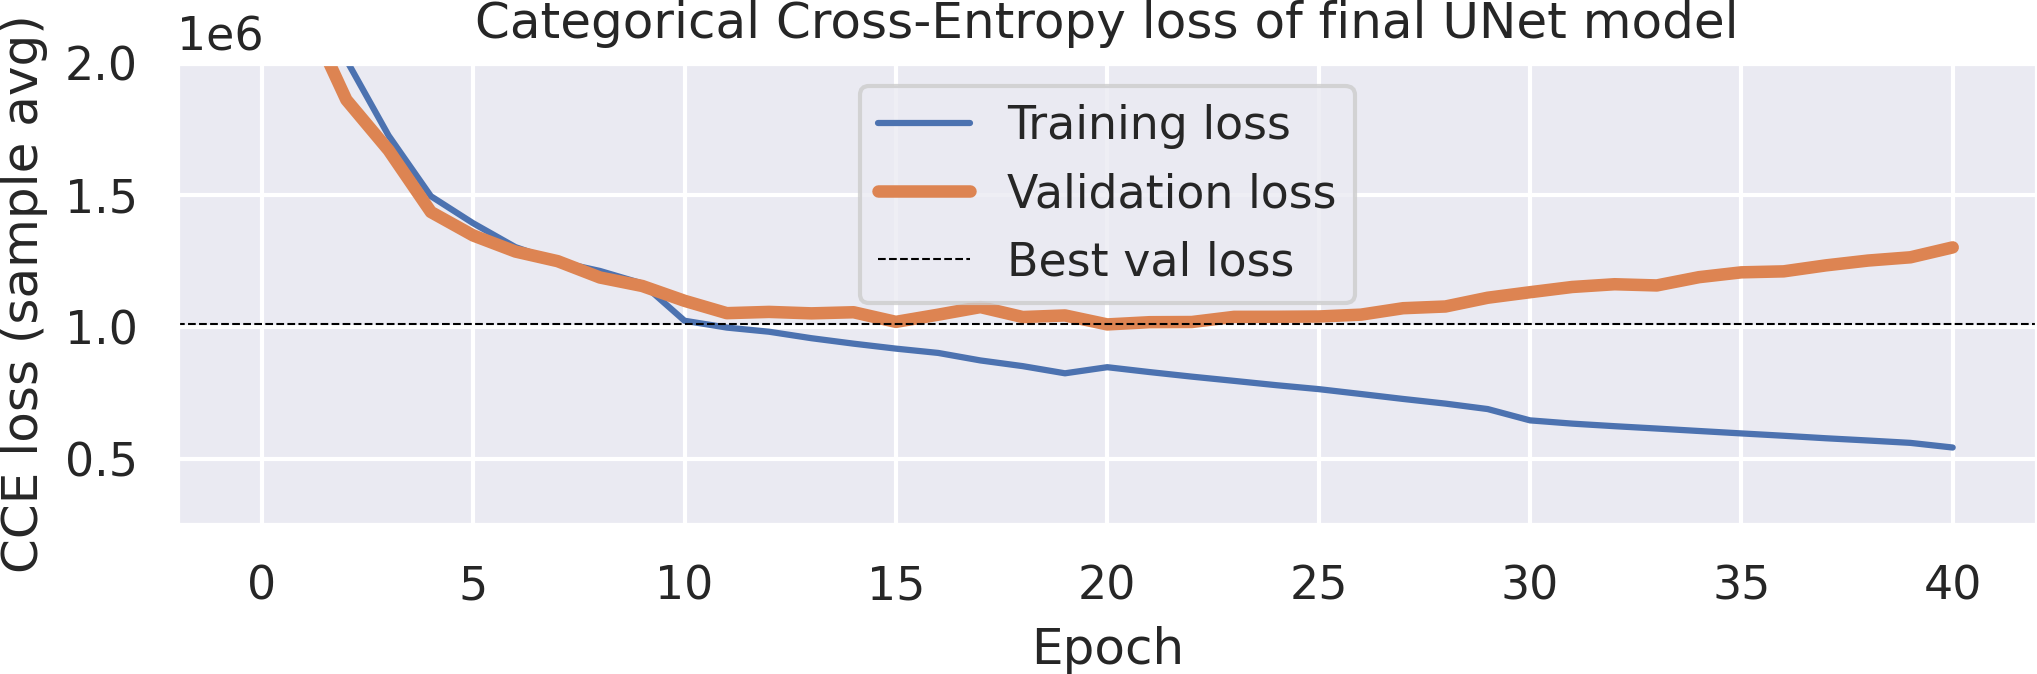
\includegraphics[width=.9\textwidth]{unet_loss.png}
	\caption{UNet model loss by epoch.}
\end{figure}

In addition to having a good loss, it's considerably better at the task of image segmentation than the baseline model

\begin{figure}[h]
	\begin{subfigure}{.5\textwidth}
		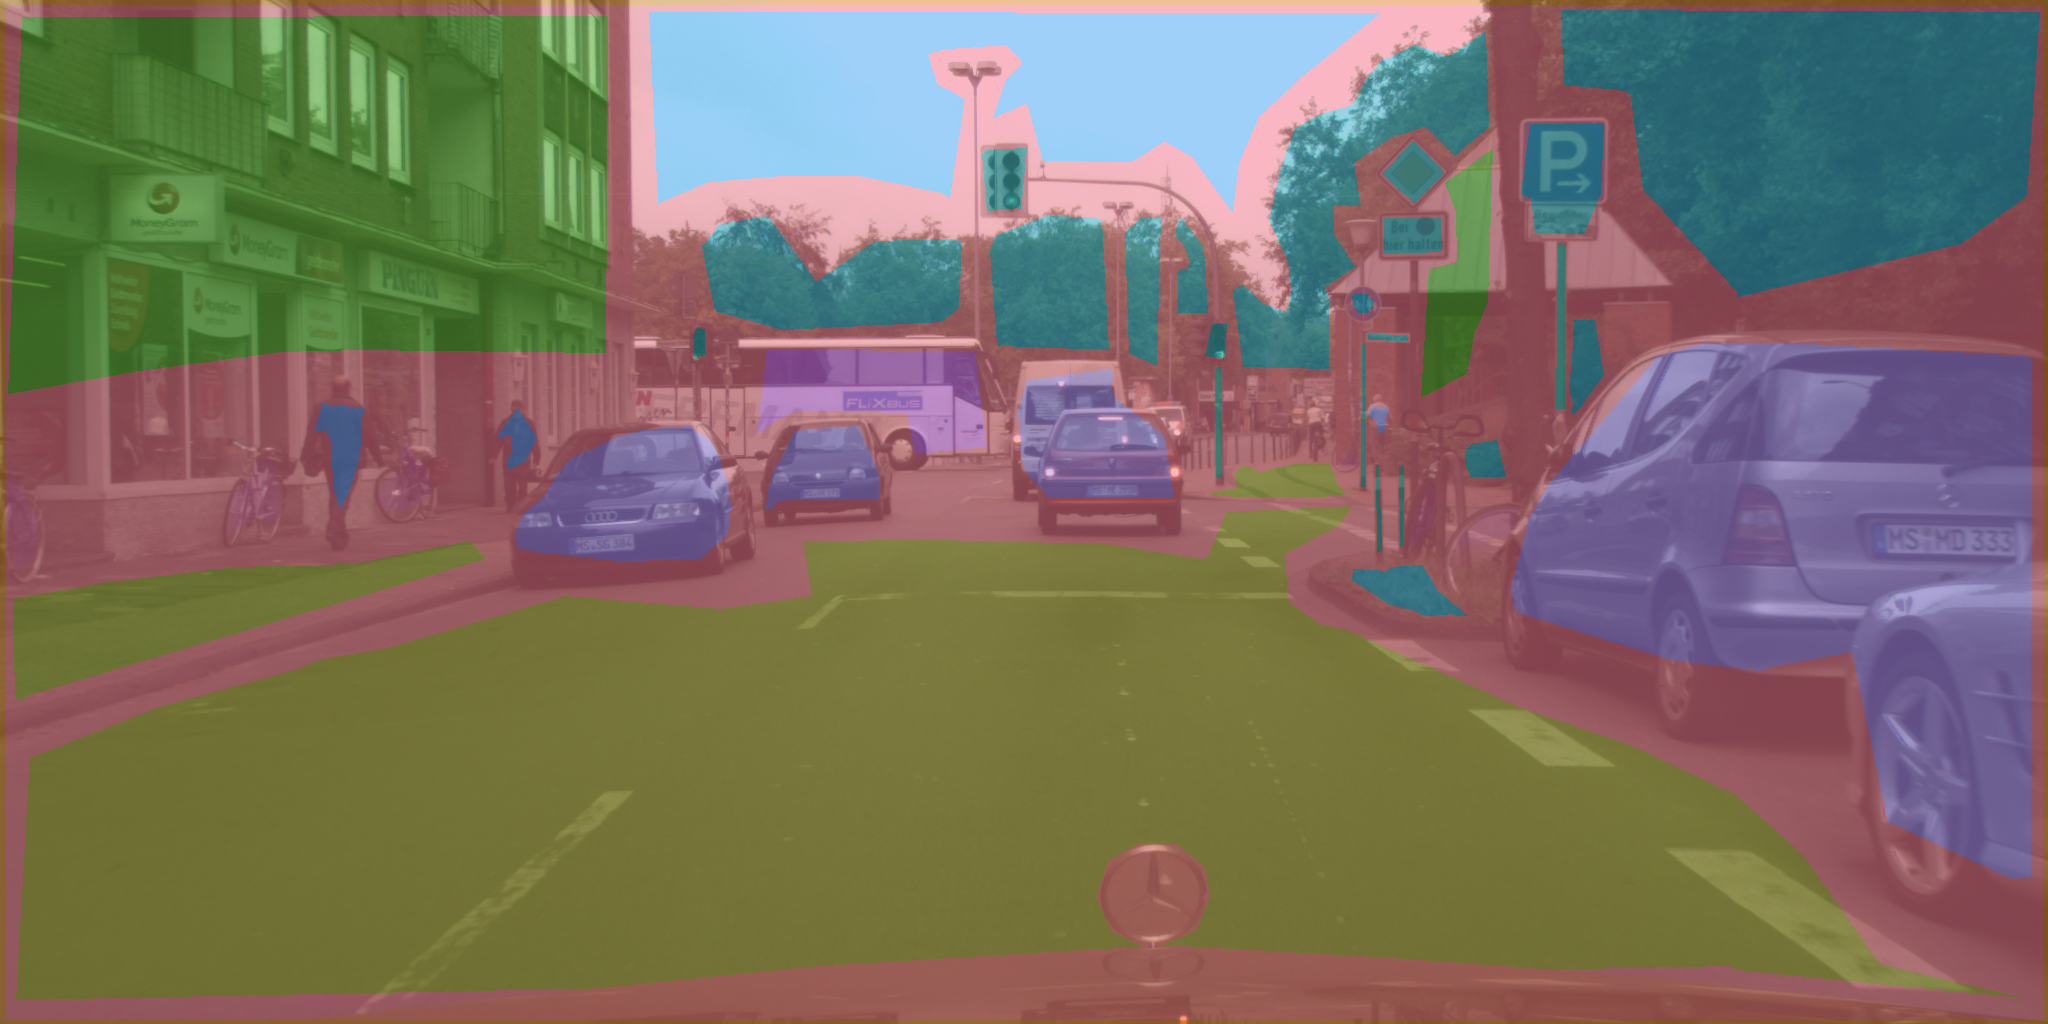
\includegraphics[width=\textwidth]{city_images/unet_gt_pic.png}
		\caption{Ground truth}
	\end{subfigure}
	\begin{subfigure}{.5\textwidth}
		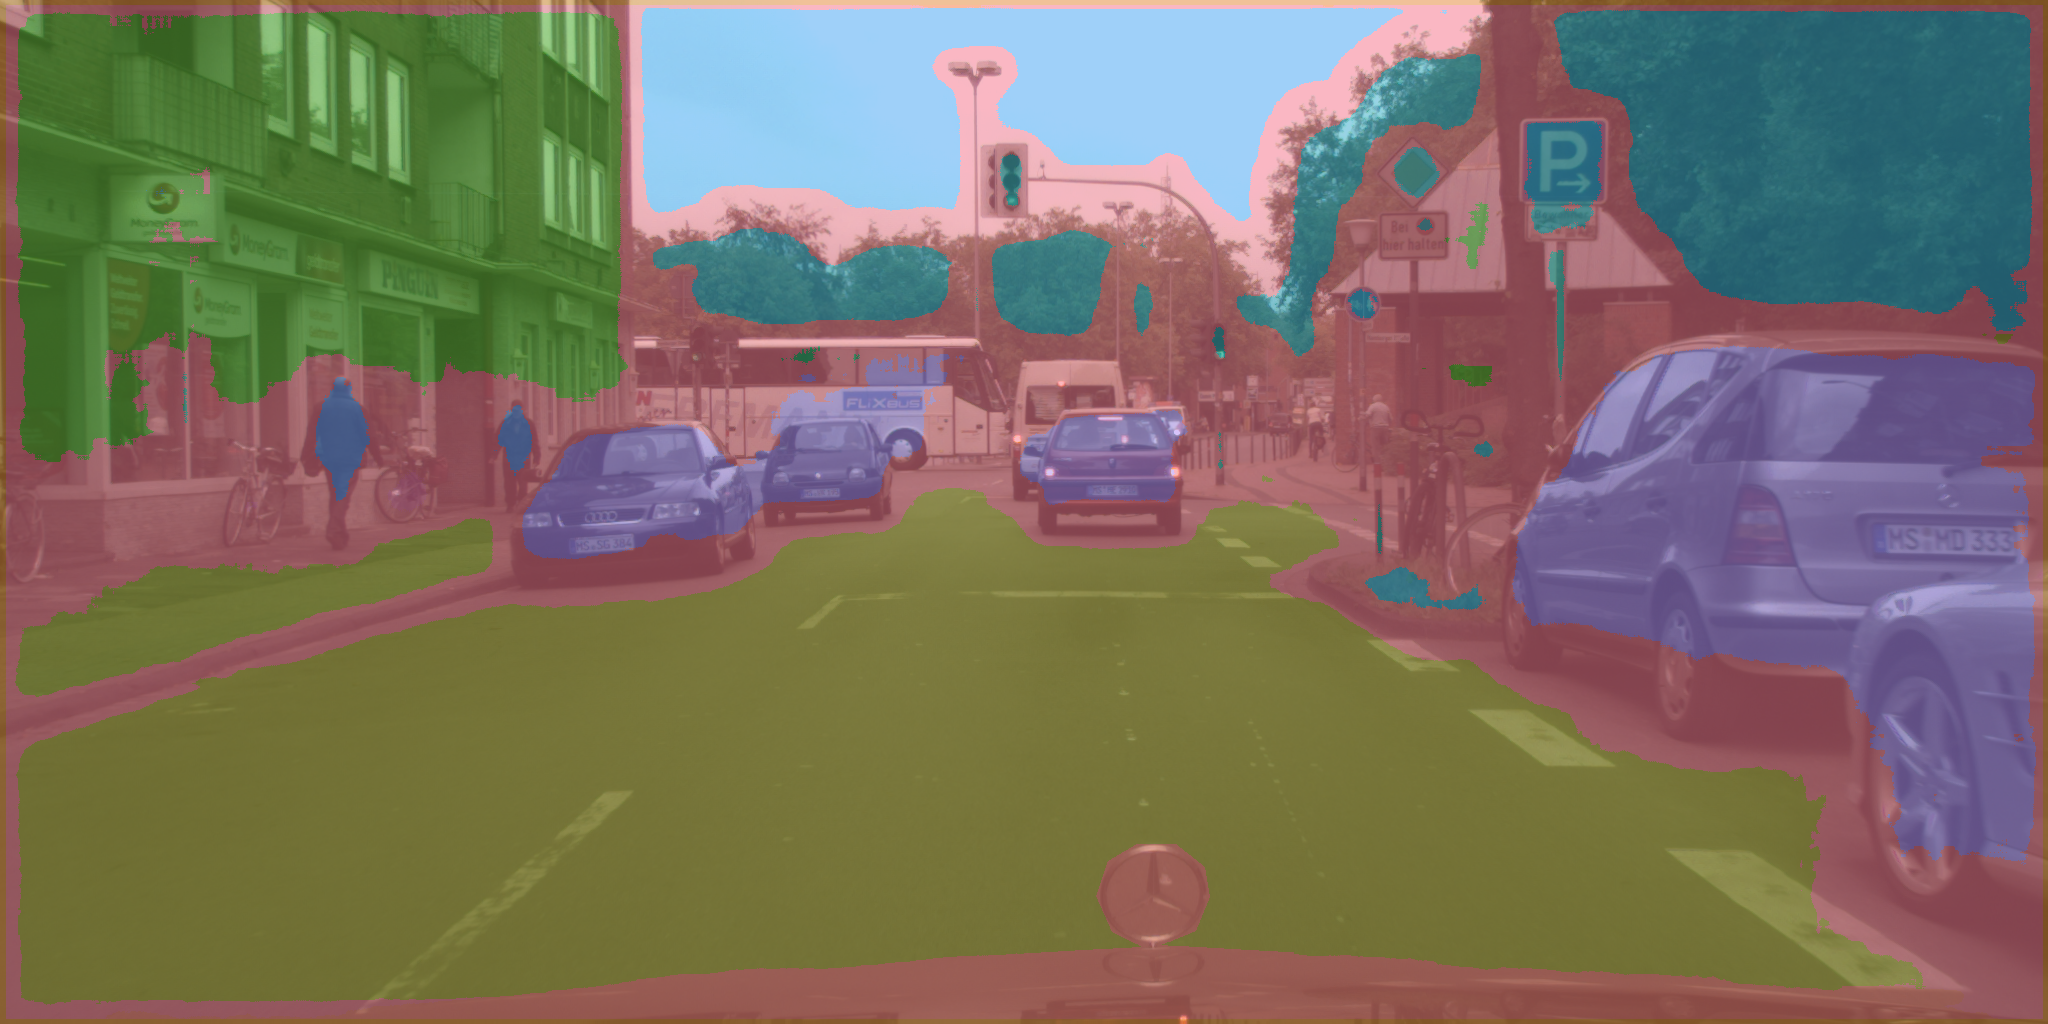
\includegraphics[width=\textwidth]{city_images/unet_pic.png}
		\caption{Result of the enhanced UNet model.}
	\end{subfigure}
	\caption{Example result with a picture in the city of Munster.}
\end{figure}

Here we can observe that the blockiness from the previous model is gone, and the filled parts are properly filled.
This is a result of how deep the encoder and decoder is, which allows it to generalise better over large patches, and of the skip connections passing data with different resolution from different parts of the encoder.

Many of the ``mistakes'' done by this model are actually caused by the arbitrariness of the coarse dataset of CityScapes.
As explained in the Reflections, this is one of the reasons why it might have been a better idea to work in the fine dataset instead.

\newpage{}

\subsection{Enhanced Model 2: Swin2}
\begin{scriptsize}
	\vspace{-\parskip}
	\url{https://wandb.ai/mfixman-convolutional-team/work/runs/wspszqbr}
	\hfill{} Wandb tag: \texttt{enhanced\_swin2}
\end{scriptsize}

The Swin2 model has the lowest validation loss of the three models.
The dropout makes it overfit late and slowly; the best loss is found only after 30 epochs, and ever after overfitting the training loss drops slowly.

\begin{figure}[h]
	\centering
	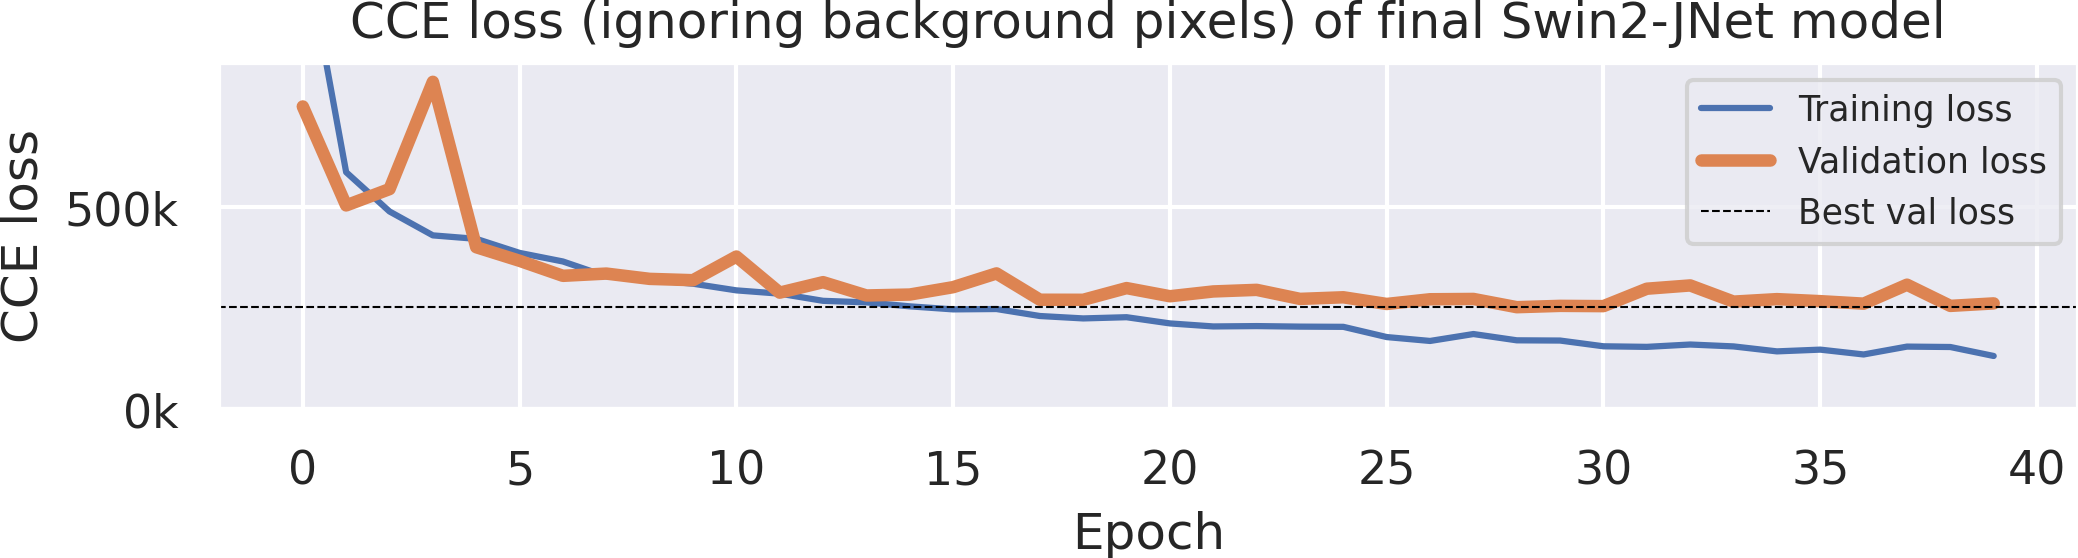
\includegraphics[width=.9\textwidth]{swin2_loss.png}
	\caption{Swin2-JNet loss by epoch.}
\end{figure}

The pre-trained weights in the transformer encoder seem to capture a lot of relevant picture information, which is later trained and used in the decoder.
This shows the promise of transfer learning: by only requiring to learn small but relevant details of the image, we can achieve a good loss in just a bit of training.

\begin{figure}[h]
	\begin{subfigure}{.5\textwidth}
		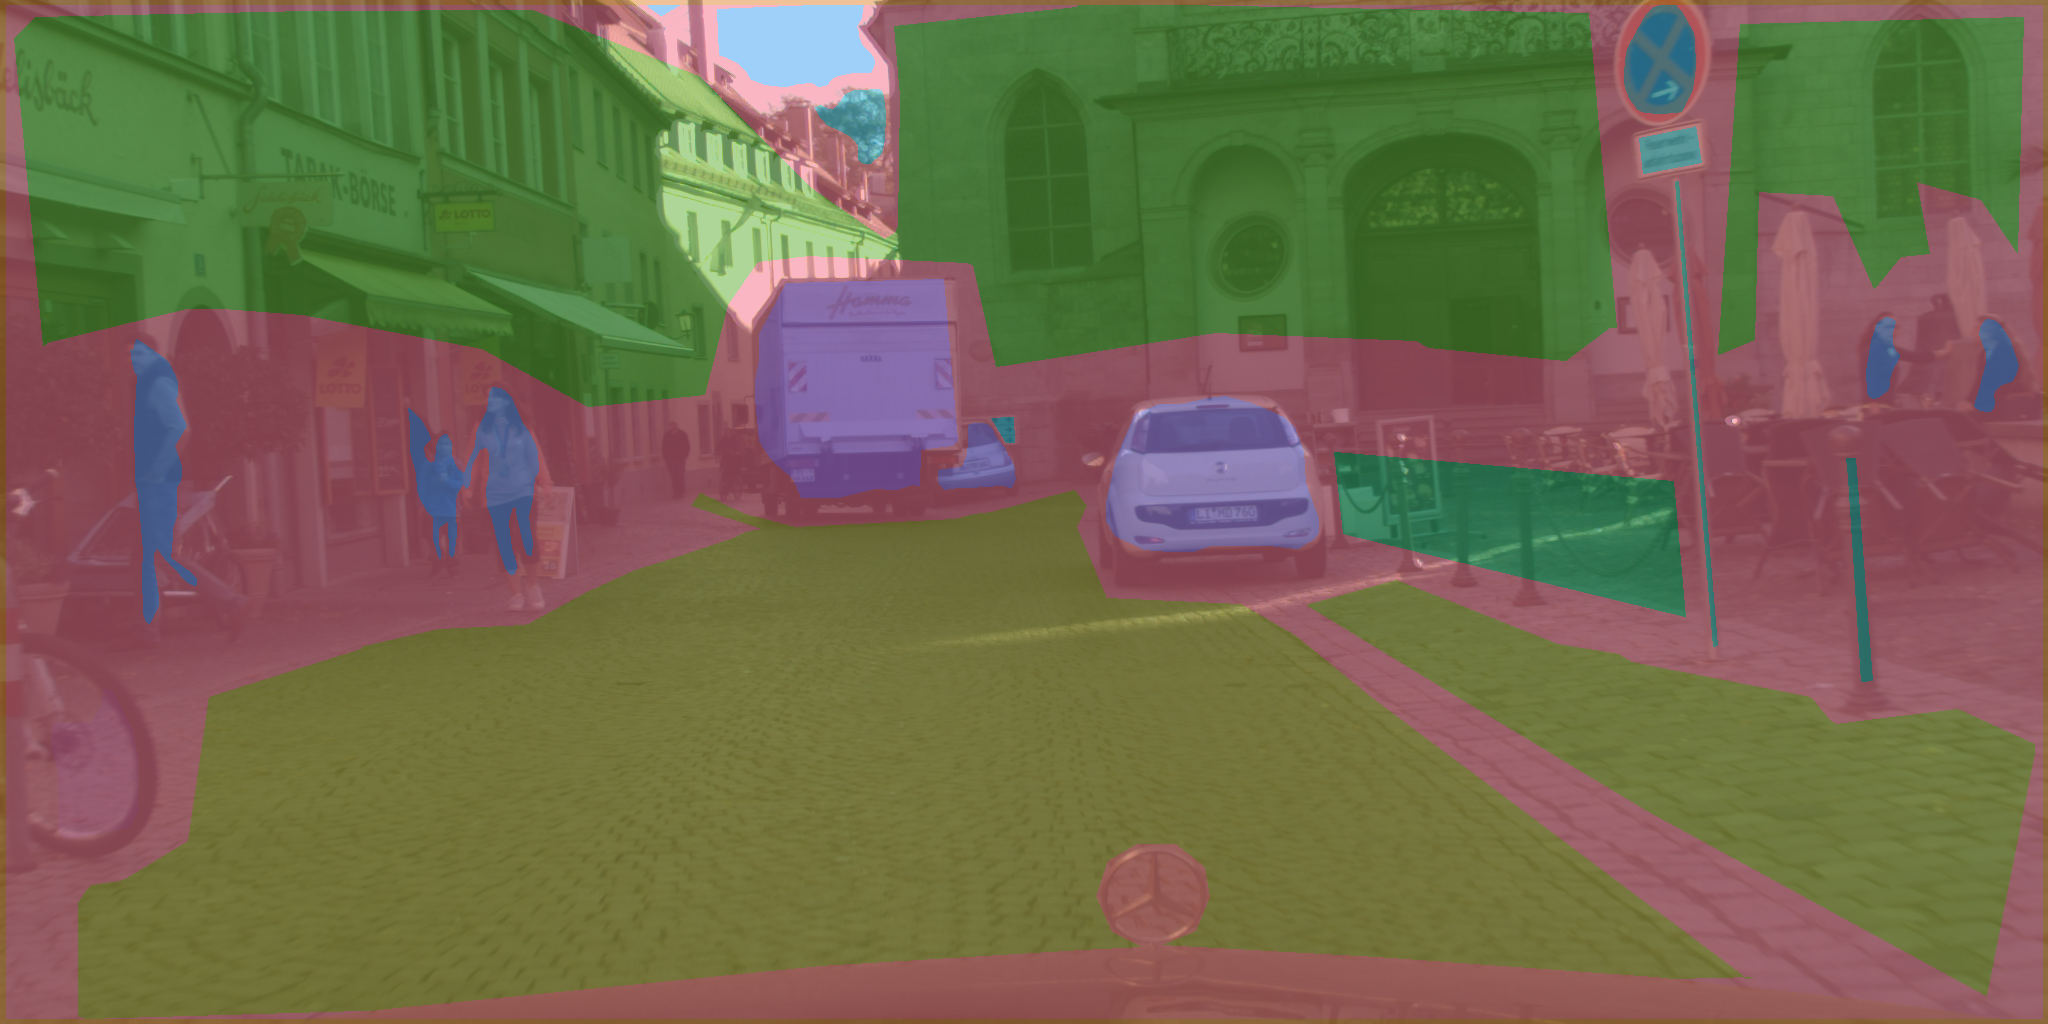
\includegraphics[width=\textwidth]{city_images/swin2_gt_pic.png}
		\caption{Ground truth}
	\end{subfigure}
	\begin{subfigure}{.5\textwidth}
		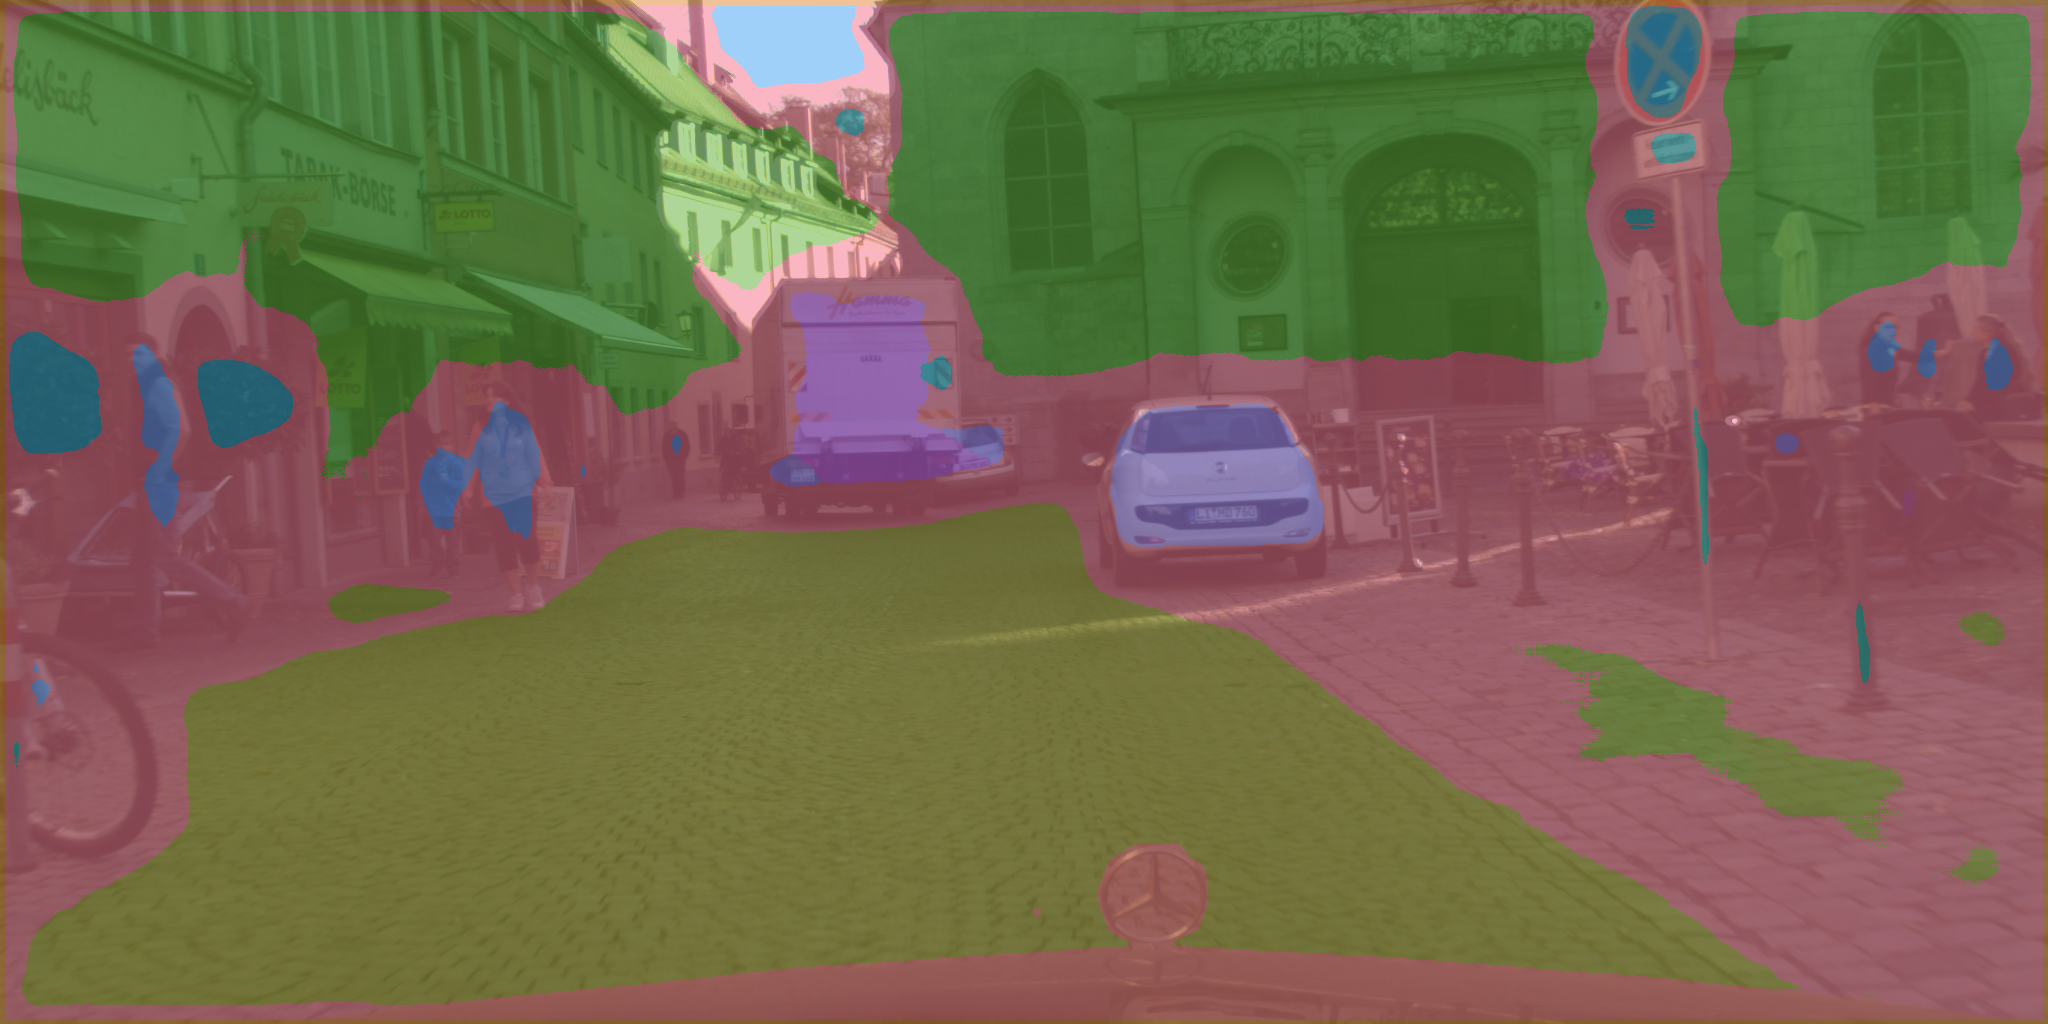
\includegraphics[width=\textwidth]{city_images/swin2_pic.png}
		\caption{Result of the enhanced Swin2-JNet model.}
	\end{subfigure}
	\caption{Example result with a picture in the city of Lindau.}
\end{figure}

While the CCE metrics are better, the results seem slightly worse and less practical than the ones in the UNet enhanced model.
For example, some classes hardly appear while many other ones appear in ``splooges'' of class.

This is likely due to the pre-trained model not being able to capture the subtleties of these specific scene, since they were trained on other kinds of images.

\newpage{}

\subsection{Comparisons}
\label{comparisons}
